\section{Evaluation}

\noindent This section reports the evaluation of \lm. Note that all datasets, scripts, and findings are available on the project website~\cite{cellsecinspector2025}. Implementations and 3GPP specifications used for evaluations are introduced in Appendix~\ref{append:implementation-datasets}. 

\subsection{Research Question}
To evaluate the performance of \lm, we answer the following research questions. 

\noindent $\diamond$ \textbf{RQ1:} Can \lm identify new vulnerabilities in 3GPP specifications?  \\
\noindent $\diamond$ \textbf{RQ2:} How does \lm compare with the state-of-the-art approach in vulnerability discovery effectiveness? \\
\noindent $\diamond$ \textbf{RQ3:} How effectively does SCA preserve procedural information? \\
\noindent $\diamond$ \textbf{RQ4:} What's the conversion rate from candidate violations to confirmed vulnerabilities?\\
\noindent $\diamond$ \textbf{RQ5:} What is \lm's runtime performance? 


\subsection{RQ1: New Vulnerabilities}
\label{subsect:rq1_new_vulnerabilities}
\begin{table*}[t]
\centering
\caption{Summary of new vulnerabilities }
\vspace{-0.1in}
\label{tab:new_vulnerabilities}
\scriptsize

\scriptsize
\setlength{\tabcolsep}{2pt}
\renewcommand{\arraystretch}{1.05}

\begin{tabular}{
|>{\raggedright\arraybackslash}p{0.9cm}
|>{\raggedright\arraybackslash}p{2.2cm}
|>{\raggedright\arraybackslash}p{4.1cm}
|>{\raggedright\arraybackslash}p{2.0cm}
|>{\raggedright\arraybackslash}p{2.55cm}
|>{\raggedright\arraybackslash}p{4.5cm}|
}


\hline
\multicolumn{1}{|c|}{\multirow{2}{*}{\textbf{Spec\#}}}
& \multicolumn{1}{c|}{\multirow{2}{*}{\textbf{Vulnerability}}} 
& \multicolumn{1}{c|}{\multirow{2}{*}{\textbf{Description}}} 
& \multicolumn{2}{c|}{\textbf{PoC Validation}} 
& \multicolumn{1}{c|}{\multirow{2}{*}{\textbf{Root cause}}} \\
\cline{4-5}
& & 
& \textbf{Validation Setup}
& \textbf{Experimental Result}
& \\
\hline

\multirow[t]{2}{=}{\raggedright
TS 24.501\newline
v16.8.0~-- \newline
v20.0.0$^\dagger$}
& V1: Multi-USIM Problematic Reachability 
& For MUSIM devices, active traffic on one SIM can prevent the other SIM from receiving paging, which an attacker can exploit to disrupt reachability
& U.S. carrier networks;\newline Samsung S24,\newline Samsung S21
& Repeated attacker calls to SIM1 prevented SIM2 from ringing across tested carrier combinations
& Specification and implementation gap for shared-transceiver MUSIM devices, where reliable paging monitoring for the inactive SIM is not guaranteed \\
\cline{2-6}

& V2: Emergency Session Teardown via Forged Signaling to Victim
& Unprotected emergency REGISTRATION and SIP signaling enable MitM injection that terminates emergency sessions
& srsRAN/srsEPC with Linphone IMS with a controlled emergency session setup
& Forged RRC RELEASE or SIP CANCEL terminated the victim's emergency session
& A threefold design weakness in emergency services: unprotected emergency NAS messages, acceptance of unauthenticated RRC RELEASE, and unprotected SIP signaling \\
\hline

TS 23.501\newline
v16.8.0~--\newline
v20.2.0$^\dagger$
& V3: Vulnerable DNS-Based PLMN Discovery over Non-3GPP Access
& In non-3GPP access, an attacker can use forged DNS responses to redirect a UE to malicious infrastructure before any security context is established
& Controlled Wi-Fi network; \newline Samsung S24,\newline Moto G Stylus 5G
& DNS poisoning blocked legitimate N3IWF/ePDG access and non-3GPP registration
& Unauthenticated DNS-based PLMN discovery over untrusted pre-attachment links enables network misdirection attacks \\
\hline

TS 24.229\newline
v16.8.0~--\newline
v20.0.0$^\dagger$
& V4: Privacy Exposure via Over-Disclosed VoIMS Signaling Headers
& Over-disclosed SIP and SDP headers expose device, user identity, and IMS infrastructure information during VoIMS signaling
& U.S. carrier networks; \newline Samsung S21, \newline Pixel 5
& SIP traces exposed private information
& The text-based SIP signaling design largely increases the risk of transmitting headers with private information \\
\hline

TS 24.301\newline
v16.8.0~--\newline
v20.0.0$^\dagger$ 
& V5: Exploitable CS-Fallback Initiation
& An attacker sniffs an unprotected extended service request and injects a forged SERVICE REJECT (with EMM cause 39 and T3442). It can trap the victim in a long throttling timer
& srsRAN/open5GS SDR testbed; \newline Samsung S24,\newline Moto G Stylus 5G
& Devices accepted forged SERVICE REJECT and stopped CSFB call setup until T3442 expired
& Specifications allow SERVICE REJECT to be processed without ciphering or integrity protection as a fail-safe mechanism, enabling attackers to inject unauthenticated rejection messages \\
\hline

\multirow[t]{2}{=}{\raggedright
TS 38.331\newline
v17.0.0~--\newline
v19.3.0$^\dagger$}
& V6: Access Trap via Access Barring Factor
& Rogue base station advertises restrictive barringFactor in SIB1/SIB2, causing UEs to suppress MO access attempts and refrain from initiating RRC connection establishment
& RF-shielded srsRAN, srsEPC testbed; \newline Samsung S24,\newline Moto G Stylus 5G
& Devices self-blocked access after receiving SIB2 with ac-BarringFactor set to 0
& UAC policies are broadcast via unauthenticated SIB messages before security is established, creating a pre-authentication trust gap \\
\cline{2-6}

& V7: Rogue Base Station RRC RESUME Blackhole
& By exploiting unauthenticated RRC RESUME procedure, a rogue gNB traps the victim UE in a continuous loop of connection failures
& RF-shielded gNB setup; \newline Samsung S21, \newline Moto G Stylus 5G
& Devices were attracted to the rogue gNB and repeatedly failed RRC RESUME
& Cell selection and reselection occur at the RRC layer before a protected AS channel is established, and the mechanism does not account for resume failures \\
\hline

\multicolumn{6}{|l|}{$\dagger$ The latest 3GPP specification version available at the time of submission.}  \\
\hline
\end{tabular}
\vspace{-0.11in}
\end{table*}





Among the well-studied TS~38.331, TS~24.501, and TS~24.301, \lm uncovers 5 new vulnerabilities.
Beyond these three specifications, we further apply \lm to TS~23.501 (System architecture for the 5G System (5GS)) and TS~24.229 (IP multimedia call control protocol based on Session Initiation Protocol (SIP) and Session Description Protocol (SDP); Stage 3) to demonstrate the extensibility of \lm beyond commonly studied NAS and RRC specifications. 
Considering that validating each finding requires substantial human effort, \lm analyzes only one selected section from TS~23.501 and TS~24.229, respectively; \lm identifies two additional vulnerabilities from selected sections. 
Table~\ref{tab:new_vulnerabilities} summarizes all 7 newly identified vulnerabilities with the precise description of the vulnerability, how we conduct the proof-of-concept validation, and the root cause analysis. All 7 findings were validated through controlled experiments using U.S. carrier networks or SDR-based testbeds. 


\noindent 
\textbf{Not every violation flagged by \lm is ultimately reported as a confirmed vulnerability here for two reasons.}
(1) \ul{Some flagged issues cannot be experimentally examined due to the missing support in operational infrastructure. Nevertheless, some flagged issues reflect the same concerns raised by domain experts through 3GPP Change Requests (CRs) before the real-world deployment.}
For example, since Release~17, TS~23.501 introduces the Unavailability Period mechanism to help the network manage unreachable states of NTN (non-terrestrial networks) UEs. 
The specification defines how the AMF determines the loss-of-coverage schedule, including the Start of Unavailability Period and the Unavailability Period Duration. 
However, it does not fully specify the UE-side handling of these configurations, despite their direct impact on paging reception, access stratum operation, and power-saving behavior. 
This creates a potential design loophole: an NTN UE and the AMF may operate with inconsistent Unavailability Period settings, which can disrupt mobility procedures and trigger transient connectivity failures and unnecessary re-registration attempts. 
Unfortunately, we did not observe support for the Unavailability Period mechanism in either operational infrastructure or SDR-based platforms. 
Importantly, after reviewing CRs used by 3GPP to create revised versions of specifications, we found that this out-of-sync Unavailability Period issue was also raised by Samsung in CR~5614~\cite{netovate_cr_search}. 
However, the proposed change does not fully eliminate the inconsistency risk. 
This alignment with an independently reported CR confirms the value of \lm's findings, even when full experimental validation is not feasible. 
Consequently, we submit these potential issues to GSMA and 3GPP rather than reporting them as confirmed vulnerabilities. 
(2) \ul{Confirmed vulnerability reporting requires substantial human effort to investigate identified issues and run validation experiments.} 
Although \lm is extensible to a broad range of 3GPP standards, in this work, we focus on a subset of specifications to demonstrate \lm's effectiveness in discovering new vulnerabilities. 

We next present V1 and V2 in detail below as representative examples, including introductions of vulnerabilities, proof-of-concept validations, and root cause \& lessons learned discussions. The remaining V3--V7 vulnerabilities are elaborated in Appendix~\ref{append:new_vulnerabilities_v1_v7} following the same structure.




\subsubsection{V1: Multi-USIM problematic reachability}



\vspace{-0.1in}
\begin{figure}[H]
    \centering
    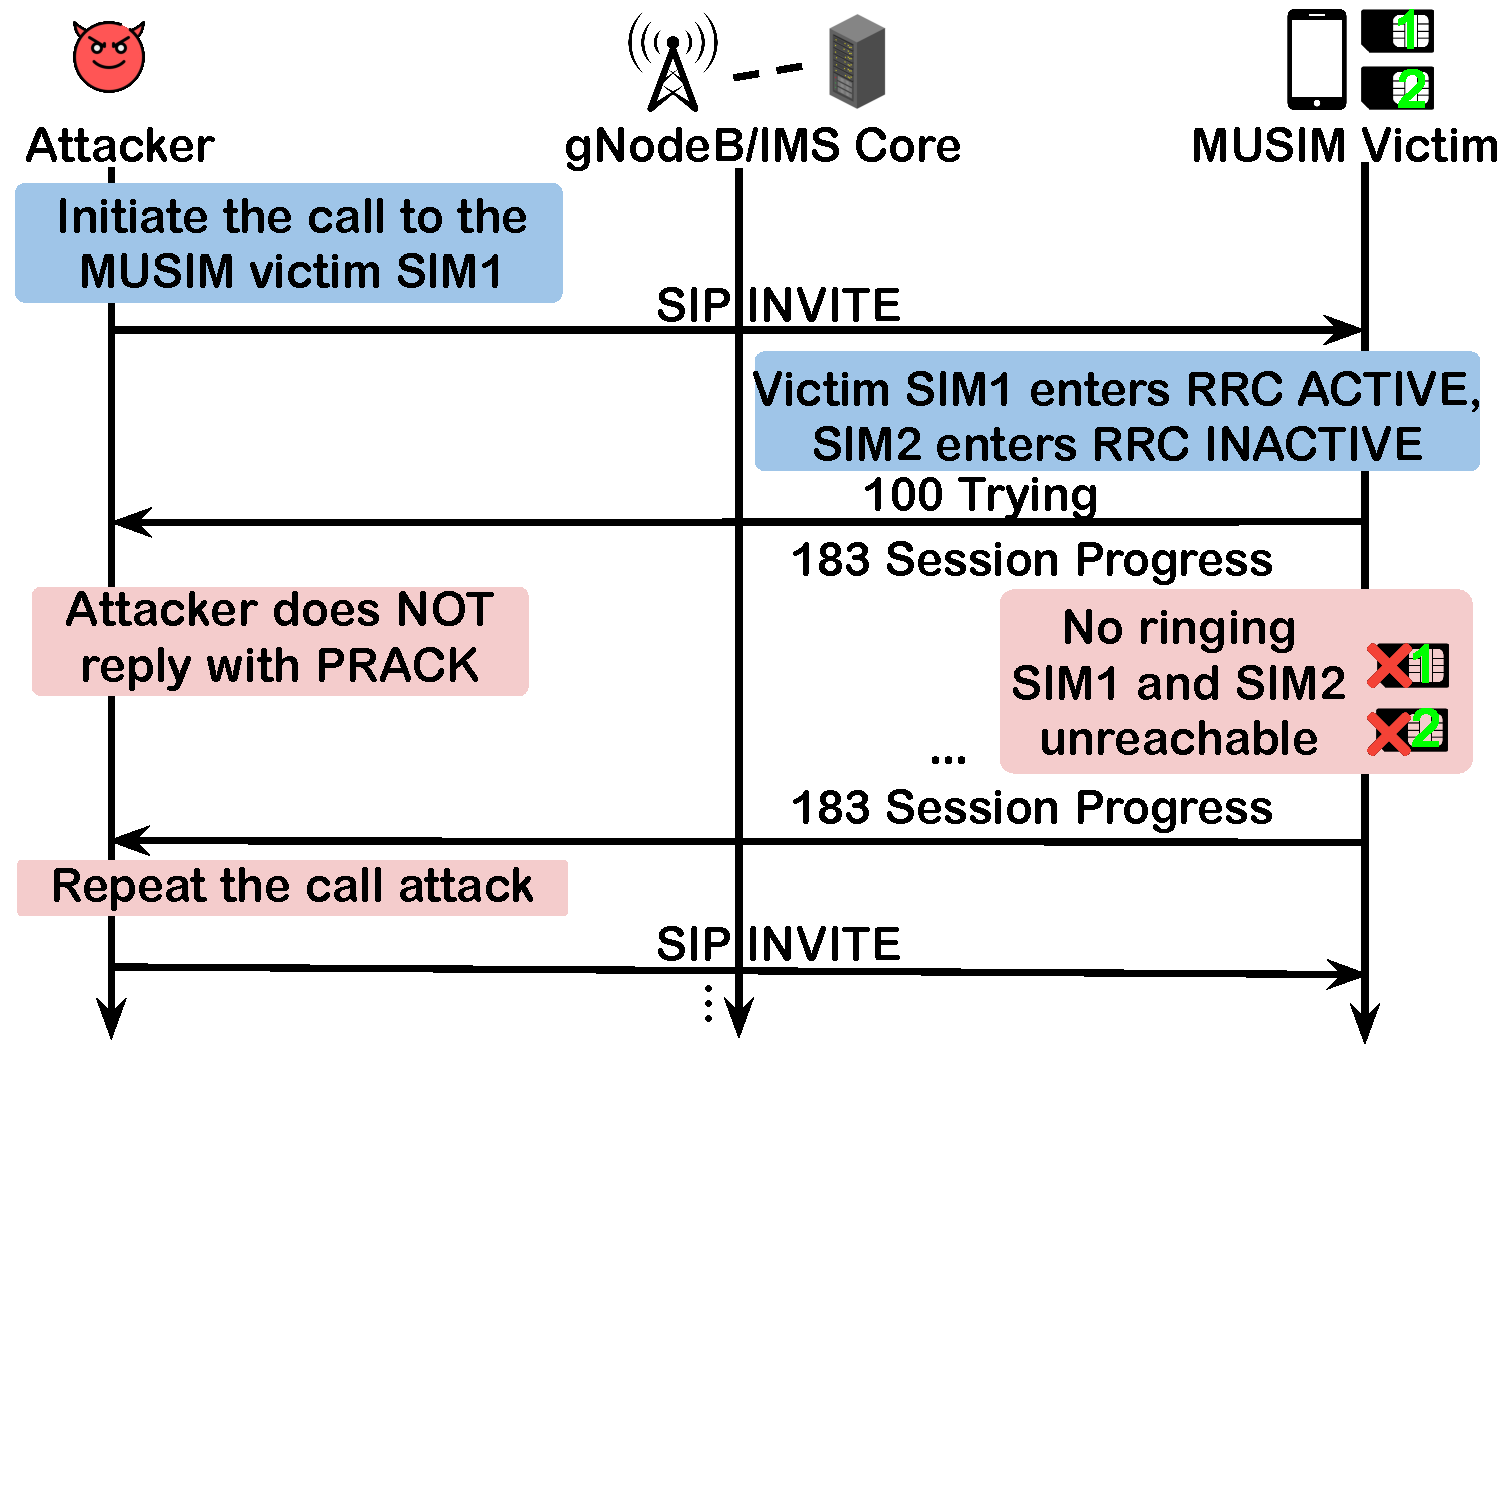
\includegraphics[page=1,width=0.8\linewidth]{pic/New_Vulnerabilities.pdf}
    \vspace{-0.1in}
    \caption{Multi-USIM Problematic Reachability}
    \label{fig:musim-dos}
    \vspace{-0.1in}
\end{figure}

5G introduces the RRC\_INACTIVE state to balance power efficiency with low-latency responsiveness. In this state, a UE remains in 5GMM\_CONNECTED mode while its RRC connection is suspended and its session context is stored. This design allows the UE to avoid full reconnection procedures, thereby saving energy and reducing signaling overhead. The mechanism is particularly relevant for multi-USIM (MUSIM) devices, as it allows a SIM in the RRC\_INACTIVE state to quickly restore its session to respond to a paging request. This appears to be a reasonable approach, especially for addressing paging collisions~\cite{3gpp2022multisim} by enabling the SIM to quickly receive the message before the request times out. 






However, in practice, most modern UEs (e.g., iPhone, Samsung Galaxy, Google Pixel) operate as Dual SIM Dual Standby, sharing a single RF transceiver. Under this hardware constraint, the design is not robust: when the transceiver is fully occupied by SIM1, SIM2 cannot monitor paging occasions or process paging requests. Despite the fact that paging includes a coarse paging cause (e.g., voice, data), the inactive SIM can still miss paging occasions and must rely on network re-paging, creating an exploitable reachability gap.




\noindent $\diamond$ {Proof-of-concept Attack.}  The victim is a MUSIM user with two SIMs on a commodity off-the-shelf (COTS) phone. 
The attacker aims to make both SIM subscriptions of the victim persistently unreachable. It assumes that at least one of the victim’s SIM numbers can be obtained from publicly available sources, such as social networking platforms, enterprise contact directories, or leaked customer databases. 
With this minimal knowledge, the attacker can launch a stealthy DoS attack against both SIMs.  

\vspace{-0.1in}
\begin{table}[H]
\centering
\caption{Multi-USIM DoS attack results}
\vspace{-0.1in}
\label{tab:dual_sim_ringing_data}
\small
\begin{tabular}{l l l c}
\hline
\textbf{Phone} & \textbf{SIM1} & \textbf{SIM2} & \textbf{Ringing?} \\
\hline
Samsung S24 & OP-I & OP-II  & x \\
Samsung S24 & OP-I & OP-I   & x \\
Samsung S24 & OP-I & OP-III & x \\
Samsung S21 & OP-I & OP-II  & x \\
Samsung S21 & OP-I & OP-I   & x \\
Samsung S21 & OP-I & OP-III & x \\
\hline
\end{tabular}
\end{table}

As illustrated in Figure~\ref{fig:musim-dos}, the attack proceeds as follows.
The attacker first initiates a call to SIM1, which establishes an active RRC connection for SIM1 and forces SIM2 into RRC INACTIVE. To avoid alerting the victim, the attacker can leverage the ghost call attack~\cite{lu2020ghost,wang2021insecurity}, preventing the call from ringing while keeping SIM1 trapped in the RRC ACTIVE state during the entire attack period. 
Note that, under the ghost call attack, SIM1 is also unable to receive any other incoming calls. Consequently, SIM2 remains stuck in RRC INACTIVE. All incoming paging requests for SIM2 will be ignored. The device neither rings nor displays an incoming call notification. As a result, the victim UE becomes persistently unreachable through both SIM1 and SIM2, despite having two independent subscriptions.   


We validate this attack on a Samsung Galaxy S24 and a Samsung Galaxy S21. We choose these devices because both provide two physical SIM slots, which simplifies repeated experiments and SIM swapping without triggering the additional security restrictions often associated with moving eSIM profiles across devices. During the interval in which the attacker withholds \textsf{PRACK}, we use another phone to call SIM2. As summarized in Table~\ref{tab:dual_sim_ringing_data}, neither device produces a ringing notification for SIM2 on any tested carrier. Notably, this attack does not strictly require a ghost call. The attacker can also keep repeatedly calling SIM1 or maintain an ongoing connection with SIM1 to occupy the shared RF resources. Although this variant is more likely to attract the victim’s attention, SIM2 still does not receive incoming call notifications during the attack period.



\noindent $\diamond$ \textbf{Root Cause and lessons learned.} 
The root cause is a mismatch between specification assumptions and widely deployed MUSIM hardware. The 5G NAS specification~\cite{3GPP_TS_24501} implicitly assumes device capabilities that can maintain simultaneous accessibility for multiple SIMs, whereas most modern MUSIM devices share a single RF module. The specifications do not mandate mechanisms that ensure all MUSIM devices, in particular, devices with a shared transceiver, can reliably monitor and process Paging Requests. This gap enables an attacker to exploit the MUSIM paging mechanism to attack MUSIM reachability.  Mitigating this issue likely requires combined core-network and device-side enhancements in future 3GPP releases. For example, MUSIM devices could implement adaptive internal scheduling for ongoing traffic/calls and bring SIMs in RRC INACTIVE to ACTIVE for paging monitoring, rather than ignoring paging on the inactive SIM. 

\vspace{-0.10in}
\subsubsection{V2: Emergency Session Teardown via Forged Signaling to Victim} 
\noindent To ensure emergency services remain accessible to all users, 5G NAS specification TS 24.501~\cite{3GPP_TS_24501} permits UEs without valid credentials to connect. If an unregistered UE attempts to make an emergency call (e.g., 911 call), it initiates a NAS REGISTRATION REQUEST with the type set to emergency registration. Since this message may be transmitted without encryption or an established NAS security context, it opens a loophole that adversaries can monitor and use a rogue base station to send fabricated responses to the UE, enabling a man-in-the-middle (MiTM) attack. 
The exposure extends to the IMS layer: TS~24.229 permits emergency SIP signaling without authentication or IPsec protection, leaving critical emergency call-control messages vulnerable to interception and manipulation~\cite{hu2024uncovering, 10479537, inproceedings,10.1145/3599184.3599195}. 

\noindent \textbf{Is it the same vulnerability in~\cite{hu2022uncovering}?} This vulnerability is fundamentally different from previously reported vulnerabilities~\cite{hu2022uncovering}, which exploit the fact that the infrastructure accepts unverifiable emergency session requests over the IP-CAN session and suffers from improper cross-layer security binding. These are infrastructure-side logic loopholes, and operators could mitigate them by temporarily allowing duplicate emergency IP-CAN sessions. Our V2 targets a loophole in the standard-permitted emergency entry path. It enables a MiTM attack at the radio and emergency signaling layers directly targeting the UE; therefore, V2 cannot be noticed by the carrier networks.

\begin{figure}[t]
    \centering
    \includegraphics[page=2,width=0.8\linewidth]{pic/New_Vulnerabilities.pdf}
    \vspace{-0.15in}
    \caption{Emergency Session Teardown via Forged Signaling to Victim}
    \label{fig:emergency}
    \vspace{-0.21in}
\end{figure}



\noindent $\diamond$ \textbf{Proof-of-concept Attacks.}
Two proof-of-concept attacks are used to validate this vulnerability. 

\noindent \textbf{Attack 1: Forcing emergency radio session release.} 
This attack exploits the NAS registration and RRC release procedures. When an unregistered UE initiates an emergency call, it sends a NAS REGISTRATION REQUEST with the type set to emergency. Because the UE does not have a valid security context, this message is transmitted unprotected. Therefore, an attacker operating a rogue base station can capture both REGISTRATION REQUEST and the REGISTRATION ACCEPT from the legitimate network. Next, the attacker can send a forged RRC RELEASE to the UE, forcing it to tear down the ongoing radio connection for the upper emergency services. 

Due to ethical considerations, we validate this attack in a fully controlled environment rather than interacting with the operational networks or real 911 call center. Specifically, we deploy a serving network using srsRAN and srsEPC~\cite{srsran}, together with an IMS service based on the Linphone VoIP server~\cite{linphone}. Additionally, we set up another set of srsRAN and srsEPC as the attacker on the same server. We use UERANSIM~\cite{ueransim} as the victim UE. 
After the UE receives the Registration Accept, the attacker keeps sending a forged RRC RELEASE to the victim UE. In wild settings, the attacker needs to do an RF scan, detect SSB/PBCH, and read MIB/SIB1 once synchronized for sending the forged RRC message on the same downlink carrier the victim is using. 
Figure~\ref{fig:emergency} shows the victim attempts to reconnect to continue the emergency service.   
The attacker can continue sending the forged RRC RELEASE to prevent the victim from getting the radio connection.  
 


\begin{figure}[t]
    \centering
    \includegraphics[page=2,width=0.95\linewidth]{pic/RRC-1.png}
    \vspace{-.1in}
    \caption{The forged RRC Release message traps the victim UE by disconnecting it from the base station}
    \label{fig:emergency}
    \vspace{-0.25in}
\end{figure}


\noindent \textbf{Attack 2: Ghost emergency call cancellation.} 
It targets the unprotected SIP signaling for emergency voice services. In this attack, the attacker leverages the fact that the 3GPP specification permits emergency services without authentication or encryption. The attacker intercepts the unencrypted SIP INVITE and spoofs a forged SIP CANCEL message, deceiving the emergency UE that the emergency call session has been legitimately terminated. We validate this attack using the aforementioned in-house setting for ethical considerations. After observing the unencrypted SIP INVITE, the attacker can send a forged SIP CANCEL to the victim to cancel the call. Our result confirms that the victim's emergency call is canceled after receiving a `ghost' cancellation signaling message.   

\noindent $\diamond$ \textbf{Root Cause and Lesson Learned.} 
These attacks stem from the lack of protection in the REGISTRATION REQUEST and the design trade-offs in the emergency service procedures to guarantee universal accessibility. Together, they expose unprotected NAS and SIP signaling to attackers, making mobile users vulnerable to emergency service DoS attacks. 
The root cause is therefore threefold: (1) the omission of mandatory encryption and authentication for emergency NAS messages, (2) the acceptance of RRC RELEASE without protections, and (3) the allowance of unprotected SIP signaling for emergency voice services. Future 3GPP specification releases must revisit the emergency service procedures and incorporate mitigations that preserve accessibility without sacrificing security. For instance, lightweight integrity-protection mechanisms could be mandated for emergency signaling, ensuring messages cannot be silently modified. Different from~\cite{hu2022uncovering}, our proposed attacks target emergency UEs; therefore, they are harder to be noticed by carriers.



\subsection{RQ2: Vulnerability Discovery Comparison}
Beyond discovering new vulnerabilities, it is important to understand how \lm performs relative to prior art. 
Accordingly, we compare \lm with the state-of-the-art approach in terms of vulnerability discovery effectiveness, which is intended to assess whether \lm can have a better coverage of security flaw identification in 3GPP specifications. As discussed in Section~\ref{sect:related}, some existing approaches~\cite{chen2021bookworm,chen2023sherlock,tan2025automated} target implementation-level issues instead of detecting design flaws in 3GPP specifications. \textit{CellularLint}~\cite{rahman2024cellularlint} aims to detect sentence-level semantic conflicts in 3GPP specifications rather than finding the design vulnerabilities.  
To the best of our knowledge, \textit{Hermes}~\cite{al2024hermes} is the only comparable system that can also discover vulnerabilities from standards. To enable a fair comparison, we collect and develop a benchmark set of known vulnerabilities~\cite{shaik2015practical, 6550445, kambourakis2011attacks, lee2009detection, leong2014unveiling, kim2019touching, van2015defeating, park2016white, chlosta2019lte, 8958725, michau2016not, hussain20195greasoner, borgaonkar2018new, 8894379, chlosta20215g, hussain2019privacy, al2024hermes, hussain2018lteinspector} that are design defects from same specifications (TS~38.331, TS~24.501, TS~24.301) used by \textit{Hermes}.



As shown in Table~\ref{tab:vulnerabilities}, \textit{Hermes} can detect 22 of all 36 known vulnerabilities in 5G and 4G NAS and RRC specifications. 
After manually verifying the candidate violations flagged by \lm, we confirm that flagged violations can cover all of these KNOWN vulnerabilities.
The vulnerability discovery results show that \lm is capable of effectively modeling mobile network procedures, conducting security analysis, and identifying security threats in 3GPP specifications. Combined with the results in RQ1, \lm not only has better vulnerability discovery coverage, but also can discover new vulnerabilities. 

\noindent \textbf{Why are there more known vulnerabilities than new vulnerabilities?}
The 36 known vulnerabilities form a cumulative benchmark collected from the aforementioned prior studies over several years, whereas the 7 new vulnerabilities include only previously unreported, experimentally validated design flaws identified in this work. As clarified in RQ1, we also exclude duplicate, implementation-dependent, and unconfirmed candidates from the new-Reference Guided Connection count. 


\begin{table}[ht]
\centering
\caption{Comparison of KNOWN vulnerabilities detected by Hermes and \lm}
\vspace{-0.1in}
\label{tab:vulnerabilities}
\scriptsize
\begin{tabularx}{\linewidth}{p{.1cm} p{5.7cm} c c}
\toprule
\textbf{ID} & \textbf{Attack} & \textbf{H*} & \textbf{C**} \\
\midrule
1 & Downgrade to non-LTE network services \cite{shaik2015practical} & \cmark & \cmark \\
2 & Denying all network services \cite{shaik2015practical} & \cmark & \cmark \\
3 & Denying selected service \cite{shaik2015practical} & \xmark & \cmark \\
4 & Signaling DoS \cite{6550445, kambourakis2011attacks, lee2009detection, leong2014unveiling} & \cmark & \cmark \\
5 & S-TMSI catching \cite{kim2019touching}& \cmark & \cmark \\
6 & IMSI catching\cite{van2015defeating}& \cmark & \cmark \\
7 & EMM Information \cite{park2016white}& \cmark & \cmark \\
8 & Impersonation attack \cite{chlosta2019lte} & \xmark & \cmark \\
9 & Synchronization Failure attack \cite{8958725} & \xmark & \cmark \\
10 & Malformed Identity Request \cite{michau2016not} & \xmark & \cmark \\
11 & Neutralizing TMSI refreshment \cite{hussain20195greasoner} & \xmark & \cmark \\
12 & NAS Counter Reset \cite{hussain20195greasoner} & \cmark & \cmark \\
13 & Uplink NAS Counter Desynchronization \cite{hussain20195greasoner} & \cmark & \cmark \\
14 & Exposing NAS Sequence Number \cite{hussain20195greasoner} & \cmark & \cmark \\
15 & Cutting off the Device \cite{hussain20195greasoner} & \xmark & \cmark \\
16 & Exposure of SQN \cite{borgaonkar2018new} & \cmark & \cmark \\
17 & 5G AKA DoS Attack\cite{8894379} & \cmark & \cmark \\
18 & SUCI catching \cite{chlosta20215g} & \xmark & \cmark \\
19 & IMSI cracking \cite{hussain2019privacy} & \xmark & \cmark \\
20 & NAS COUNT update attack \cite{al2024hermes} & \cmark & \cmark \\
21 & Deletion of allowed CAG list \cite{al2024hermes} & \cmark & \cmark \\
22 & Downgrade using ATTACH/REGISTRATION REJECT \cite{shaik2015practical} & \cmark & \cmark \\
23 & AUTHENTICATION REJECT attack \cite{8958725} & \cmark & \cmark \\
24 & DETACH/DEREGISTRATION REQUEST attack \cite{hussain2018lteinspector} & \cmark & \cmark \\
25 & SERVICE REJECT attack \cite{shaik2015practical} & \cmark & \cmark \\
26 & Denial-of-Service with RRC SETUP REQUEST attack \cite{hussain20195greasoner} & \xmark & \cmark \\
27 & Installing Null Cipher and Null Integrity \cite{hussain20195greasoner} & \cmark & \cmark \\
28 & Lullaby Attack \cite{hussain20195greasoner} & \cmark & \cmark \\
29 & Incarceration with RRC REJECT/RELEASE \cite{hussain20195greasoner} & \cmark & \cmark \\
30 & Measurement report \cite{shaik2015practical} & \xmark & \cmark \\
31 & RLF report \cite{shaik2015practical} & \cmark & \cmark \\
32 & Blind DoS attack \cite{kim2019touching} & \xmark & \cmark \\
33 & AKA bypass \cite{kim2019touching} & \xmark & \cmark \\
34 & Paging channel hijacking \cite{hussain2018lteinspector} & \xmark & \cmark \\
35 & Energy Depletion with RRC SETUP \cite{al2024hermes} & \cmark & \cmark \\
36 & V2X Message Spoofing over PC5 \cite{sedar2023comprehensive} & \xmark & \cmark \\
\midrule
\multicolumn{2}{l}{\textbf{Detected Ratio}} & \textbf{22/36} & \textbf{36/36} \\
\multicolumn{4}{l}{H*: \textit{Hermes}, C**: \lm} \\
\bottomrule
\end{tabularx}
\vspace{-0.2in}
\end{table}


\subsection{RQ3: How effectively does SCA preserve procedural information?}


SCA nodes are the core modeling representation of \lm. As introduced in Section~\ref{subsect:sca_representation}, each SCA node represents one self-contained transition using four fields. The vulnerability-discovery results in RQ1 and RQ2 demonstrate the effectiveness of \lm, but do not explain whether SCA preserves the procedural information (i.e., states, conditions, and actions) required for downstream function-chain construction and security analysis in \textit{Function Chain Builder} and \textit{SecOracle}. Because FSMs are the dominant representation used by prior specification-analysis systems, we next compare SCA nodes with the conventional FSMs synthesized by prior works. The goal of this evaluation is to isolate the contribution of SCA and examine whether SCA can better preserve the procedural information needed for downstream tasks. 



\textit{Hermes}~\cite{al2024hermes} is the closest reference system, which extracts protocol models from 3GPP specifications for security analysis. \textit{ARCANE}~\cite{tan2025automated} is also included, while its FSMs are designed for impleme-\ ntation-level model-based fuzzing rather than specification-level design-flaw analysis. All three approaches are applied to the same 5G/4G NAS and RRC specifications. Because conventional FSMs do not expose conditions and actions as explicit fields, we normalize the representations into the same four-field structure: start state, condition, action, and end state. For \textit{Hermes}, condition and action information is derived from its parsed FSM transitions. For \textit{ARCANE}, we adopt its manual approach to map its message-level transitions and information-element constraints into the same structure. We then showcase the evaluation using three metrics: quantity, completeness, and accuracy.





\begin{figure}[t]
    \centering
    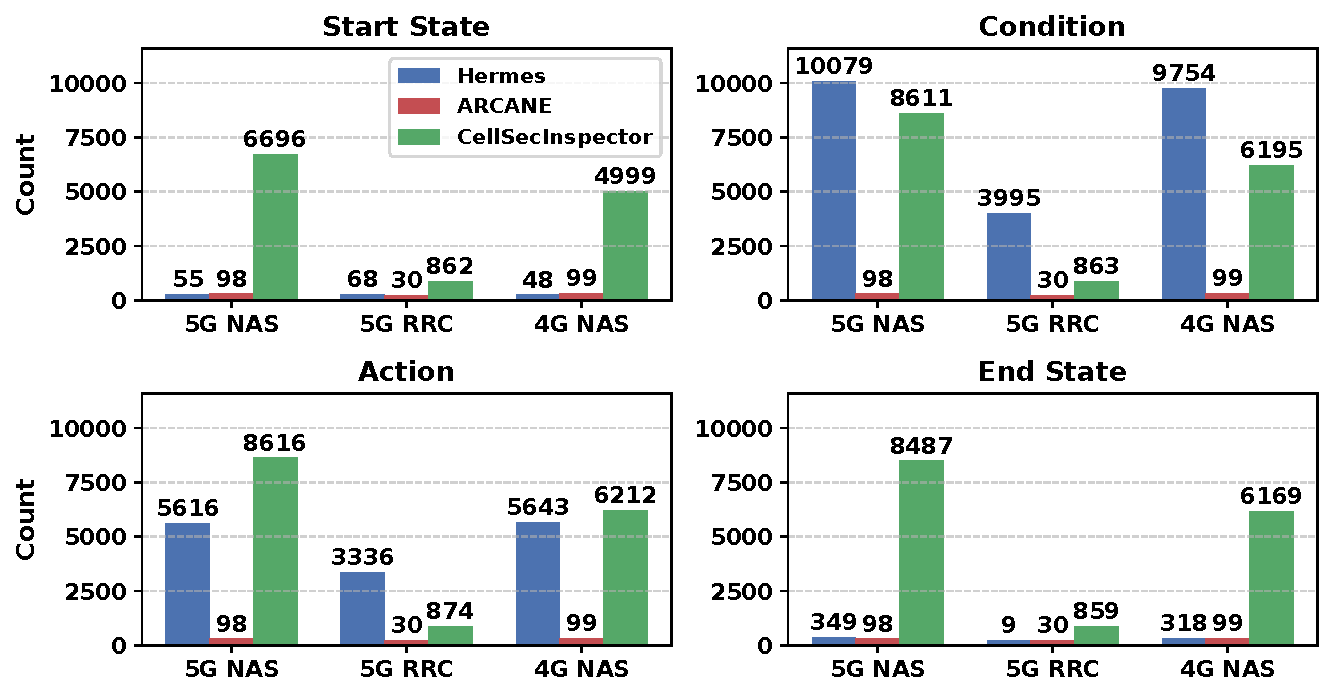
\includegraphics[width=1\linewidth]{pic/sca_statistics.pdf}
    \vspace{-.3in}
    \caption{Quantity Comparison of SCA nodes and FSMs}
    \label{fig:sca_statistics}
    \vspace{-0.1in}
\end{figure}

\noindent \textbf{Quantity.} Figure~\ref{fig:sca_statistics} shows the number of extracted fields across the three specifications. There are two key observations. (1) SCA captures substantially more start and end states than the two FSM-based approaches, indicating more derived mobile network functions from 3GPP specifications. Table~\ref{tab:sca_vs_hermes} compares an SCA node derived by \lm and an FSM transition annotated by \textit{Hermes} for a sentence `\textit{A UE enters the state 5GMM-SERVICE-REQUEST-INITIATED after it has started the service request procedure and is waiting for a response from the network.}' from TS 24.501. While the sentence does not explicitly specify the start state, \lm reasonably infers that the UE is likely in the 5GMM-REGISTERED state and correctly recognizes two sequential conditions, the action, and the end state. (2) \textit{Hermes} reports a larger number of extracted conditions and actions in 5G and 4G NAS and RRC specifications. However, it is primarily due to splitting closely connected conditions and actions within a single sentence into multiple independent entries, as shown in Table~\ref{tab:sca_vs_hermes}. This fragmentation inflates raw counts of extracted elements but fails to preserve the internal structure and logical interdependencies among conditions and actions. 


\begin{table}[t]
\centering
\caption{Comparison between an SCA node from \lm and an FSM transition from \textit{Hermes}}
\vspace{-0.1in}
\label{tab:sca_vs_hermes}
\scriptsize
\setlength{\tabcolsep}{2.8pt}
\begin{tabular}{p{0.9cm} | p{3.1cm} | p{3.9cm}}
\toprule
\textbf{Element} & \textbf{\lm (SCA Node)} & \textbf{\textit{Hermes} (FSM Transition)} \\
\midrule
\textbf{Start State} &
UE is likely in 5GMM-REGISTERED. &
\texttt{<start\_state>} A UE enters the state 5GMM-SERVICE-REQUEST-INITIATED \texttt{</start\_state>} \\
\midrule
\textbf{Condi- tion} &
After the UE has started the service request procedure AND is waiting for a response from the network. &
\texttt{<condition>} it has started the service request procedure \texttt{</condition>} \newline
\texttt{<condition>} is waiting for a response from the network \texttt{</condition>} \\
\midrule
\textbf{Action} &
UE enters the 5GMM-SERVICE-REQUEST-INITIATED state. &
N/A \\
\midrule
\textbf{End State} &
UE is in the 5GMM-SERVICE-REQUEST-INITIATED state, waiting for a response from the network. &
N/A \\
\bottomrule
\end{tabular}
\end{table}


\begin{table}[t]
\centering
\caption{
SCA completeness comparison of Hermes, ARCANE, and \lm
}
\vspace{-0.1in}
\label{tab:sca_completeness}
\scriptsize
\setlength{\tabcolsep}{2.2pt}
\begin{tabular}{p{0.5cm}lccccc}
\toprule
\textbf{Spec\#} & \textbf{Method} & \textbf{0 fields} & \textbf{1 field} & \textbf{2 fields} & \textbf{3 fields} & \textbf{4 fields} \\
\midrule

\multirow{3}{*}{24.501}
 & Hermes  & 1122 (20.1\%) & 1055 (19.0\%) & 2177 (39.1\%) & 207 (3.7\%) & 5 (0.1\%)   \\
 & CellSec & 1778 (17.1\%) & 36 (0.3\%)    & 132 (1.3\%)  & 1920 (18.4\%) & 6549 (62.9\%) \\
 & ARCANE  & 0 (0\%) & 0 (0\%) & 0 (0\%) & 0 (0\%) & 98 (100\%) \\

\midrule

\multirow{3}{*}{38.331}
 & Hermes  & 2948 (46.2\%) & 2675 (41.9\%) & 753 (11.8\%) & 1 (0.0\%) & 0 (0.0\%)   \\
 & CellSec & 321 (26.9\%)  & 11 (0.9\%)    & 1 (0.1\%)   & 7 (0.6\%) & 855 (71.5\%) \\
 & ARCANE  & 0 (0\%) & 0 (0\%) & 0 (0\%) & 0 (0\%) & 30 (100\%) \\

\midrule

\multirow{3}{*}{24.301}
 & Hermes  & 3026  (50.6\%) & 463 (7.7\%)   & 2244 (37.5\%) & 237 (4.0\%) & 6 (0.1\%)   \\
 & CellSec & 1771 (22.2\%) & 30 (0.4\%)    & 13 (0.2\%)   & 1207 (15.1\%) & 4974 (62.2\%) \\
 & ARCANE  & 0 (0\%) & 0 (0\%) & 0 (0\%) & 0 (0\%) & 99 (100\%) \\

\bottomrule
\end{tabular}
\vspace{-0.15in}
\end{table}



\noindent \textbf{Completeness.} We evaluate the completeness of state transitions. A state transition is defined to be complete if all 4 corresponding start, condition, action, and end fields can be derived and are not placeholders (e.g., ``Not specified'' or ``Not explicitly defined''). More complete fields indicate that more information is likely derived from 3GPP specifications. 

\begin{table}[t]
\centering
\caption{Expert evaluation results}
\vspace{-0.1in}
\label{tab:expert_evaluation}
\scriptsize
\setlength{\tabcolsep}{5pt}
\renewcommand{\arraystretch}{1.00}
\begin{tabular}{lccccc}
\multicolumn{6}{c}{\textbf{(a) Expert judgment of SCA nodes and FSMs}} \\
\midrule
\textbf{Method} & \textbf{Total} & \textbf{Accuracy} & \textbf{$\{a,b,c,d\}$} & \textbf{Raw Agr.} & \textbf{$\kappa$} \\
\midrule
\textit{CellSecInspector} & 3147 & 98.92\% & $\{3113,13,8,13\}$ & 99.33\% & 0.80 \\
\textit{Hermes} & 3634 & 25.23\% & $\{917,32,28,2657\}$ & 98.35\% & 0.96 \\
\textit{ARCANE} & 162 & 0.00\% & $\{0,0,0,162\}$ & 100.00\% & N/A \\
\midrule
%\multicolumn{6}{c}{} \\
\addlinespace[2.2pt]

\multicolumn{6}{c}{\textbf{(b) Expert validation of SCA node extraction across 4 models}} \\
\midrule
\textbf{Model} & \textbf{Expert1} & \textbf{Expert2} & \textbf{Avg. Acc.} & \textbf{Cohen's $\kappa$} & \\
\midrule
DeepSeek-V3.2 & 1.00 & 1.00 & 1.00 & 1.00 & \\
Qwen-Plus & 1.00 & 1.00 & 1.00 & 1.00 & \\
Qwen3-4B & 0.90 & 0.90 & 0.90 & 0.92 & \\
DeepSeek-R1-8B & 0.90 & 1.00 & 0.95 & 0.94 & \\
\midrule
\end{tabular}
\vspace{-0.26in}
\end{table}

As shown in Table~\ref{tab:sca_completeness}, it is observed that a large portion of SCA transitions contain three or four valid fields, and 62.2\%--71.5\% of the extracted transitions are fully specified across the three specifications. \textit{Hermes} extracts many partial transitions, while \textit{ARCANE} produces a much smaller set of structurally complete message-level transitions because its representation is intentionally tailored to fuzzing. These results show that SCA provides a useful balance between broad procedural coverage and preservation of the information required for downstream security analysis.






\noindent \textbf{Accuracy.} We evaluate whether an SCA node or an FSM is accurate based on two criteria: (1) evidence-grounded correctness, whether each extracted representation accurately reflects the protocol behavior described in the specification and is supported by explicit textual evidence, and (2) semantic consistency, whether the extracted representation preserves the intended meaning of the mobile network function behavior described in 3GPP specifications. Because this judgment requires domain expertise in cellular network standards, it cannot be reliably outsourced to crowdworkers. We thus ask two domain experts to independently judge whether an SCA node/an FSM is accurate. Formally, each SCA node and FSM is labeled as $v_i \in \{Pass, Fail\}$. We define that an SCA node or FSM is accurate only if both experts label it as Pass. Based on the annotations from two experts, we construct a contingency table $\{a,b,c,d\}$, where $a$ denotes Pass/Pass, $b$ denotes Pass/Fail, $c$ denotes Fail/Pass, and $d$ denotes Fail/Fail. Due to the large amount of SCA nodes and FSMs, two experts are asked to assess the SCA nodes and FSMs extracted from the selected sections, including Clause 4 of 4G NAS specification, Clause 4 of 5G NAS specification, Clauses 4 and 5 of 5G RRC specification. 
We report the acceptance rate ($a/N$), raw agreement ($(a+d)/N$), and Cohen's $\kappa$ in Table~\ref{tab:expert_evaluation} (a).





The results show that the SCA representation more consistently preserves 3GPP specification-grounded and semantically coherent protocol behaviors. The main advantage is not the use of a different label format, but the explicit binding of the start state, triggering condition, prescribed action, and end state within one transition. By comparison, FSMs from \textit{Hermes} and \textit{ARCANE} may be suitable for their own downstream tasks (i.e., parsing or fuzzing). However, both experts agree that FSMs from \textit{Hermes} and \textit{ARCANE} struggle to model the mobile network functions.

We also assess whether the accuracy of extracted SCA nodes can be affected if \core is built on different vanilla models. Four models, \textbf{Qwen-Plus-2025-12-01}, \textbf{Qwen3-4B-Instruct-2507}, \textbf{DeepSeek-V3.2 Release 2025/12/01}, and \textbf{DeepSeek-R1-Distill-Llama-8B}, are used to adapt cellular domain knowledge and extract SCA nodes. As shown in Table~\ref{tab:expert_evaluation}(b), all four models achieve high sampled accuracy, while the larger models perform best. This result indicates that the SCA formulation is transferable across different base models and larger models are preferable choices since the capability still affects extraction quality. 







\subsection{RQ4: Candidate Violation to Confirmed Vulnerability Conversion Rate}

As introduced in Sections~\ref{subsect:secoracle} and \ref{subsect:rq1_new_vulnerabilities}, not every candidate violation can be assessed and validated as a confirmed vulnerability. We therefore adopt strict, conservative criteria to measure the conversion rate from candidate violations to confirmed vulnerabilities: a candidate violation identified by \lm is classified as a confirmed vulnerability only if it satisfies the following criteria: (i) it is attributable to a standard-defined procedure; (ii) it is non-duplicate; (iii) it is not solely implementation-dependent; and (iv) it is experimentally validated when the required testing support is available. Candidates that are duplicates, implementation-dependent, or currently unverifiable due to missing operational or SDR support are not counted as confirmed vulnerabilities. 
Under these strict conservative criterion, \lm reports 90 candidate violations in TS~24.501, of which 18 are confirmed as valid design-defect instances; 62 candidates in TS~24.301, of which 15 are confirmed; 161 candidates in TS~38.331, of which 12 are confirmed; 36 candidates in the analyzed section of TS~23.501, of which 1 is confirmed; and 8 candidates in the analyzed section of TS~24.229, of which 1 is confirmed. Known vulnerabilities 22--25 in Table~\ref{tab:vulnerabilities} occur independently in both 5G and 4G specifications and are therefore counted as separate confirmed instances. 


The relatively low conversion rate is mainly caused by repeated reports of the same root cause, implementation-dependent cases, and candidates that cannot yet be validated due to limited infrastructure support. For example, identical RRC messages reused across multiple TS~38.331 procedures can generate several candidate violations corresponding to one underlying weakness. Thus, these conversion rates should not be interpreted as the accuracy of the final confirmed vulnerability set. 
Instead, they are lower-bound rates over all candidate violations produced by \lm, which narrows a large specification analysis space to a smaller set of security-relevant candidates for expert review and validation. 





\subsection{RQ5: Runtime Performance}

We measure the end-to-end processing time of key components, including \textit{SCA Representation Extractor}, \textit{Function Chain Builder}, \textit{SecOracle}, and \textit{VulnTestGenerator}. The reported runtime is measured using DeepSeek-V3.2~\cite{deepseek_v32_release_2025} via its public API through a workstation running Ubuntu 24.04 LTS with an NVIDIA RTX 4090 GPU.   
For the full specifications TS~24.501 (5G NAS), TS~24.301 (4G NAS), and TS~38.331 (5G RRC), and the selected sections of TS~23.501 (5G system architecture) and TS~24.229 (IMS signaling), the \textit{SCA Representation Extractor} derives 10,415, 7,995, 1,195, 1,253, and 320 SCA nodes in 17.36, 13.33, 1.99, 2.09, and 0.53 hours, respectively. The \textit{Function Chain Builder} is the primary runtime bottleneck. 
It takes approximately 60 days, 30 days, 4 days, 0.44 days, and 0.03 days to construct 11,273, 6,943, 222, 83, and 6 function chains, respectively, with an average of 5.46 seconds per analyzed SCA pair. Approximately 99\% of this time is spent identifying semantic and causal connections. Reference Guided Connection substantially reduces the candidate search space. \textit{Without it, exhaustive all-pair analysis becomes infeasible in our experimental setting. For example, on TS~24.501, our design reduces the estimated runtime from approximately 18.78 years ($10,415^2 \times \frac{5.46~\text{sec}}{3600 \times 24 \times 365} = 18.78 ~\text{years}$) to 60 days.} The \textit{SecOracle} and \textit{VulnTestGenerator} together complete vulnerability analysis and test case generation in 17.54, 10.80, 0.35, 2.10, and 0.54 hours for the five specifications, respectively. 

\noindent\textbf{Scalability limit.}
Although \lm improves the scalability of specification analysis, corpus-wide 3GPP analysis remains computationally challenging. Directly linking all SCA nodes across hundreds of specifications would create a prohibitively large pairwise search space, and the resulting semantic and causal checks would dominate runtime. Therefore, corpus-wide analysis requires further efforts, such as our reference-guided design that reduces the process from years to days, to achieve with limited computational resources. A practical deployment should prioritize security-critical specifications, such as the TS~23/24 control-plane families; \lm should be executed in parallel to boost the runtime performance. Overall, the current results demonstrate the feasibility of automated security analysis for large, security-critical specifications while identifying scalability as an important direction for future work.  


 





